\documentclass{article}

% --- load packages ---
\usepackage[margin=1in]{geometry} % change the margins
\usepackage{amsmath} % useful math environments and commands like align
\usepackage[colorlinks,bookmarks,bookmarksnumbered,allcolors=blue]{hyperref} % hyperlinks between references
\usepackage[justification=centering]{caption}
\usepackage{graphicx}  % include images
\usepackage[table,xcdraw]{xcolor}
\usepackage[caption=false]{subfig} % subfigures.  false option prevents conflicts in caption styling with other packages
\usepackage{booktabs} % better tables
\usepackage[capitalise]{cleveref} % better referencing. uses cref.
\usepackage[section]{placeins} % sometimes useful to prevent figures from floating out of a section
\usepackage{cite} % handles multiple citations in one command better
\usepackage{doi} % allow correct hypderlinking of DOIs
\usepackage[normalem]{ulem}
\usepackage{float}
\usepackage{minted}
\usepackage{pdfpages}
\usepackage{tikz}
\usepackage{csvsimple}
\usepackage{adjustbox, lipsum}
\usepackage{setspace}
\usetikzlibrary{tikzmark}

\useunder{\uline}{\ul}{}
\newcommand{\wide}{0.7\linewidth}


\begin{document}
\singlespacing
\title{Computing Derivatives Report}
\author{Landon Wright}
% put in \date{} if you don't want a date to appear, or enter a specific date, otherwise default is today's date.
\maketitle

\section{Scaling issues}
% What do you learn here

\section{Derivative integration}
\subsection{Implementation}
The implementation of the different differentiation methods was performed very similarly for each method and the associated code can be seen in Section \ref{sec:code}. For each gradient to be calculated a simple function was created that accepted the location where the gradient should be determined, the value of the function/stress at that location and the objective function.  This function and its associated output was then added to the obj or con function in the OptimizeTruss.m file.  For simplicity an obj and con function was created for each of the different differentiation methods.  Each of the functions created follows the same pattern. The Data file is called to import the required data into the scope of the function and a array of zeros is created to hold the gradient.  The function then enters a loop where each of the design variables are perturbed as required, the objective/stress is calculated, the derivative approximation is carried out, and the approximation is stored in the gradient array.
\subsection{Forward Difference}
% how
% difficulties
The Forward difference is perhaps the simplest numerical differentiation method to calculate The derivative is calculated:
\begin{equation}
\frac{df}{dx} = \frac{f\left(x + \Delta x\right) - f(x)}{\Delta x}
\end{equation}
This simplicity however comes at the cost of accuracy as it is the least accurate of all the methods implemented. We can estimate the error of this method as:
\begin{equation}
Error = \left(\frac{2\epsilon + \xi}{\Delta x}\right) \pm \frac{1}{2} \frac{d^2 f}{dx^2}\Delta x
\end{equation}
I found this method to be exceptionally simple to implement.  I did have some challenge understanding how to properly account for the inequality constraints, but that was present in all three methods not unique to forward difference.  I was also unable to obtain approval of my gradients from the fmincon checkgradients function.  The discrepancies often were found to be on the order of $3e^{-6}$ which is slightly above fmincon's tolerance of $1e^{-6}$ however this error did not seem to prevent the function from converging to the optimum value.
% expected error
% how calculated
\subsection{Central Difference}
% how
% difficulties
The central difference method adds slight difficulty to that of forward difference in that it requires perturbing the function both forward and backward.  It is calculated:
\begin{equation}
\frac{df}{dx} = \frac{f\left(x + \Delta x\right) - f\left(x - \Delta x\right)}{2\Delta x}
\end{equation}
This added complexity comes with the benefit of being much more accurate.  The error for this method is calculated as follows:
\begin{equation}
Error = \left(\frac{\epsilon + \xi}{\Delta x}\right) \pm \frac{1}{6} \frac{d^3 f}{dx^3}\Delta x^2
\end{equation}
Because the truncation term of the error equation is raised to the square of the perturbation the resulting error is much smaller than what is present in the forward difference method.  I didn't face much difficulty in implementing this method due to its similarity to the forward difference method.
% expected error
% how calculated
\subsection{Complex-step}
% how
% difficulties
The Complex step method is quite similar to the forward difference method however in place of perturbing the function in the real number space it is perturbed in the complex number plane.  As such it is calculated as follows:
\begin{equation}
\frac{df}{dx} = \frac{Im\left[f\left(x - i\Delta x\right)\right]}{\Delta x}
\end{equation}
The real benefit of this method is seen in the calculation of the error:
\begin{equation}
Error = \left(\frac{\epsilon}{\Delta x}\right) \pm \left|\frac{1}{6} \frac{d^3 f}{dx^3}\Delta x^2\right|
\end{equation}
Because there is no error due to subtractive cancellation this method can be used with arbitrarily small $\Delta x$ values.  As a result the error with this method is often simply machine epsilon. The main difficulty that I experience with this method was that the absolute value function is not defined for imaginary numbers.  While this is not an exceptionally complicated thing to fix it did require the reevaluation of how to implement the stress constraints when evaluating the gradient. 
% expected error
% how calculated

\section{Derivative errors}
% What are they?
\begin{table}[H]
	\begin{center}
	\caption{Errors in derivatives as starting point (\textit{note:}
  because the complex step method is known to be accurate within the limits of
  the computer it was used as the standard for the actual derivative. As such
  its derivative error is shown as 0.)
	}
	\label{tab:errors}
	\noindent\adjustbox{max width=\textwidth}{%
		\csvautotabular{meanerrors.csv}}
	\end{center}
\end{table}
% Are they in line with expectations?
The derivative errors shown in Table \ref{tab:errors} represent the error of the different methods with respect to the actual derivative.
 Because the error in the complex step method converges to zero within the limits
 of the computer as the step becomes small it was used with a step size of $1e^{-30}$ as the reference for the actual derivative of the function,
 as such its error values in the table are shown to be 0.
 The other values in the table are in line with the expected errors of the method.
 We expect that forward difference have a larger error than central difference,
 and we further expect that the complex step method have the smallest error.

% How decided on good perturbation?
To determine the perturbation values for the different methods the step size
for the complex step method was first set to a very small value of $1e^{-30}$
The error of the other two methods were then calculated and the step sizes of
those methods was adjusted until the errors were minimized.

% Merits of different approaches?
The various methods all have different benefits and challenges.
Forward difference is the simplest of the implemented methods and as such requires the least processing power to implement.
Further because it requires a somewhat larger step to provide accuracy due to it's truncation error it is an effective method to use on noisy data.
Central difference is a more accurate method than forward difference, however this accuracy is obtained at the cost of function calls.
Lastly the complex-step method is equivalent to the forward difference method with respect to the number of function calls,
and it further benefits from the fact that because the values are calculated in the complex number plane the method does not suffer from the effects of subtractive cancellation.
As a result the step size can be driven quite small to minimize the truncation error that is inherent,
however because of the computation of numbers in the complex plane this method does still require substantial computation resources when compared to the forward difference method.

\section{Tabulated results}
% Table showing:
% Number of function calls and iterations to reach optimum for each method
% Time of execution for each method (if possible)
% Stopping criterion given by MATLAB (why it terminated, final objective value)
\begin{table}[H]
	\caption{Results of 50 fmincon trials using the sqp algoritm}
	\label{tab:efficincy}
	\noindent\adjustbox{max width=\textwidth}{%
		\csvautotabular{output-sqp.csv}}
\end{table}

% What do you learn from the above?
The results shown in Table \ref{tab:efficincy} provide some insights into the
different benefits of the methods implemented as well as some insight into the
sqp algorithm that was used to find the optimum.  The most obvious thing that we
can see in the table is that complex step method is the slowest to compute.  We
can also comfirm that the central difference method requires significantly more
function calls than the other two methods.  The number shown in the table is
however less than the double of forward difference that we expected.  This is
due to the fact that the forward difference and complex step methods both
require 11 function calls to determine the values and either gradient at a given location. The
complex step method however requires 21 function calls to determine the values and either
gradient.  These numbers correspond to 30 evaluations for any of the three
methods.


\section{Automatic Differentiation}
\subsection{Method of implementation}
% How does the method work?
The code for the implementation of this method can be found in Section \ref{ADcode}
% How does AD differ from other methods?

% \begin{table}[H]
% 	\caption{Quasi-Newton progression}
% 	\centering
% 	\noindent\adjustbox{max width=\textwidth}{%
% \begin{tabular}{|r|c|c|c|c|c|}
% 	\hline
%   % \noindent\adjustbox{max width=\textwidth}{%
%   &\bfseries Start-value & \bfseries Value & \bfseries Step-direction & \bfseries Step-len & \bfseries Function-calls
%
%   \csvreader[head to column names]{output3.csv}{}%
%   {\\\thecsvrow & (\a, \b, \c)& \d & (\e, \f, \g) & \h & \i}
%   \\\hline
% \end{tabular}}
% \end{table}

\section{Matlab Code}\label{sec:code}
\subsection{Changes to OptimizeTruss.m}\label{sec:optTrussChanges}
\begin{minted}[xleftmargin=10pt,linenos]{matlab}
function [f, grad] = obj_fd(x)
[f, ~, ~] = objcon(x);
grad = fd_obj_grad(@Truss, f, x);
end
function [c, ceq, grad, eqgrad] = con_fd(x)
[~, c, ceq] = objcon(x);
eqgrad = [];
grad = fd_con_grad(@Truss, c, x);
end

function [f, grad] = obj_cd(x)
[f, ~, ~] = objcon(x);
grad = cd_obj_grad(@Truss, f, x);
end
function [c, ceq, grad, eqgrad] = con_cd(x)
[~, c, ceq] = objcon(x);
eqgrad = [];
grad = cd_con_grad(@Truss, c, x);
end

function [f, grad] = obj_cs(x)
[f, ~, ~] = objcon(x);
grad = cs_obj_grad(@Truss, f, x);
end
function [c, ceq, grad, eqgrad] = con_cs(x)
[~, c, ceq] = objcon(x);
eqgrad = [];
grad = cs_con_grad(@Truss, c, x);
end
\end{minted}

\subsection{Forward Difference Implementation}\label{sec:fd_code}
\inputminted[xleftmargin=10pt,linenos]{matlab}{fd_obj_grad.m}
\inputminted[xleftmargin=10pt,linenos]{matlab}{fd_con_grad.m}

\subsection{Center Difference Implementation}\label{sec:cd_code}
\inputminted[xleftmargin=10pt,linenos]{matlab}{cd_obj_grad.m}
\inputminted[xleftmargin=10pt,linenos]{matlab}{cd_con_grad.m}

\subsection{Forward Difference Implementation}\label{sec:cs_code}
\inputminted[xleftmargin=10pt,linenos]{matlab}{cs_obj_grad.m}
\inputminted[xleftmargin=10pt,linenos]{matlab}{cs_con_grad.m}
\subsection{Driver}
% \inputminted[xleftmargin=10pt,linenos]{matlab}{fminunDriv.m}
\subsection{Automatic Differentiation Code}\label{ADcode}

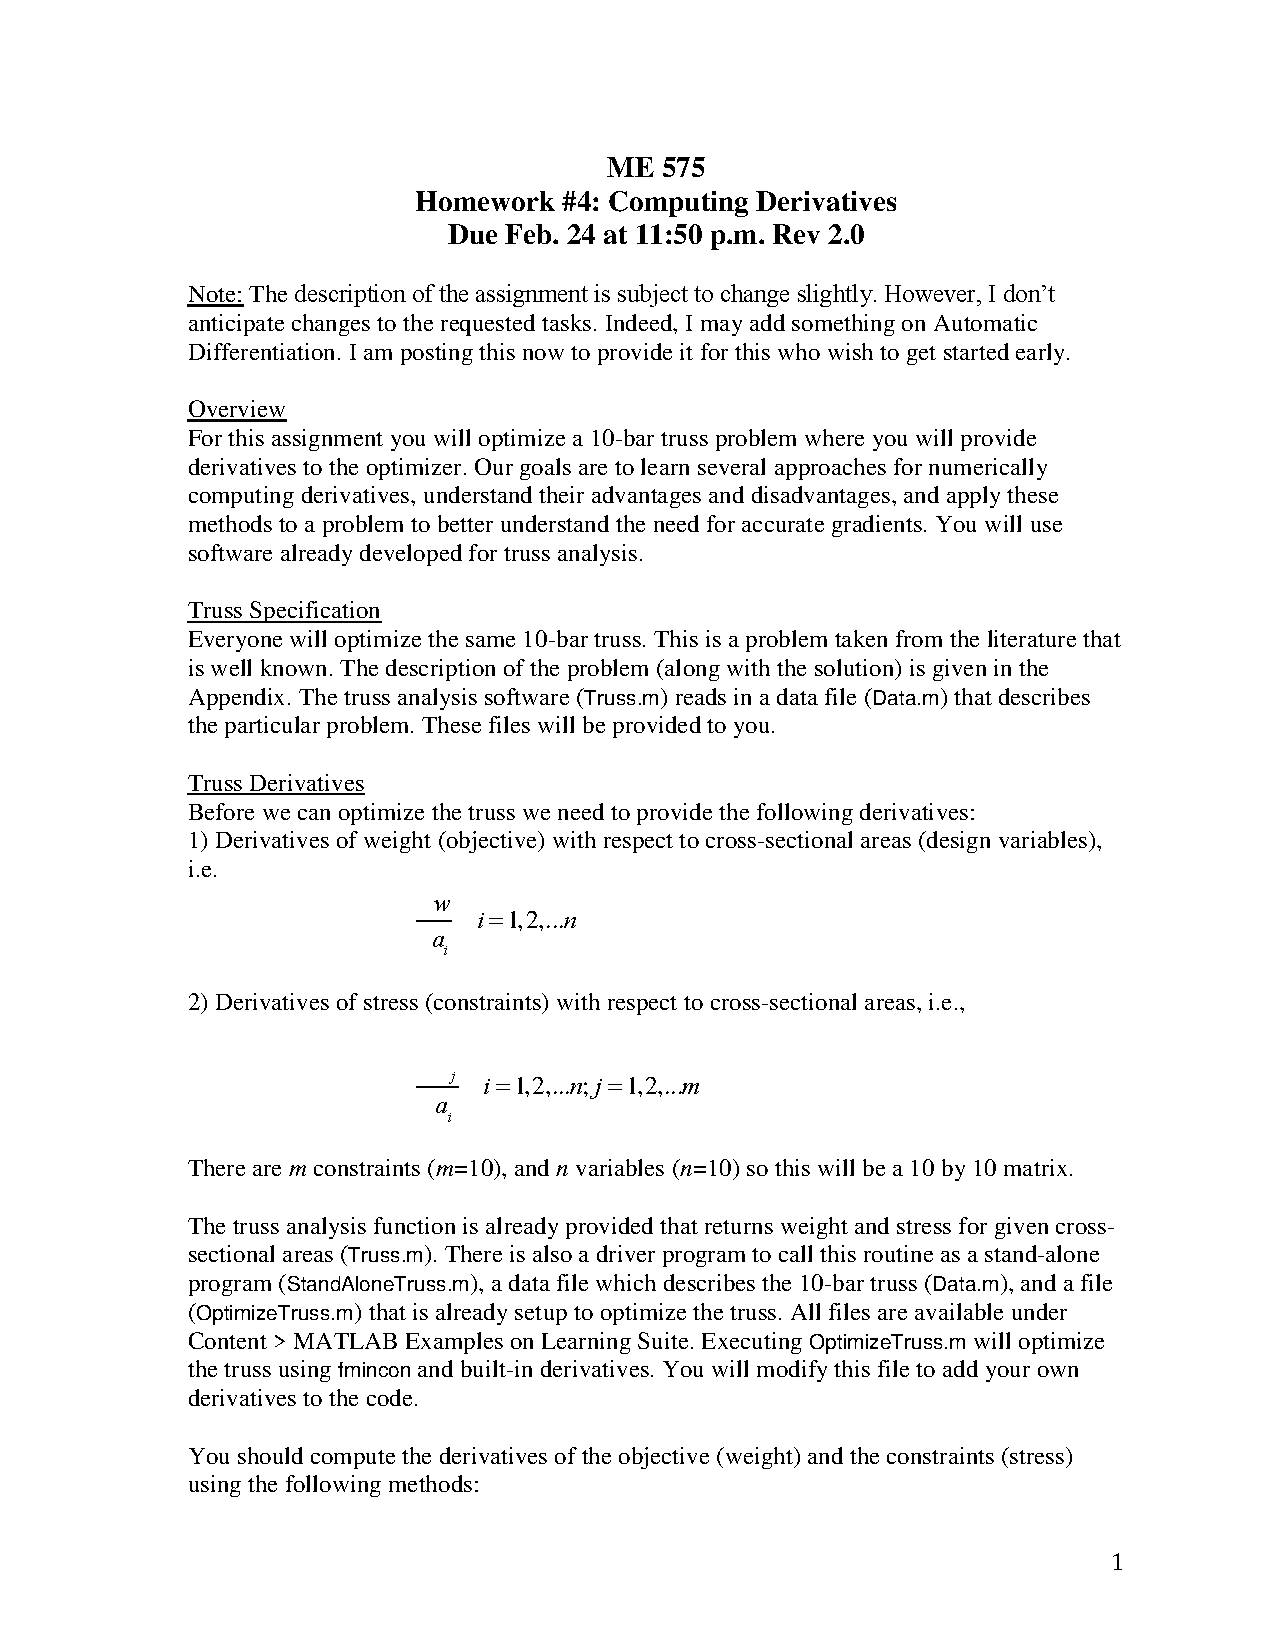
\includepdf[pages=-, pagecommand={}]{HW4.pdf}
\end{document}
